% =====================================================================
% Aletheia: A Compound AI System for NZ-US Cross-Border Tax-Contract Audit
%
% COMPSCI 703 Final Report.  Format: NeurIPS 2026 LaTeX style
% (the current Overleaf NeurIPS template ships neurips_2026.sty).
%
% Overleaf usage:
%   1. Start from the official "Formatting Instructions For NeurIPS 2026"
%      Overleaf template — it already includes `neurips_2026.sty`.
%   2. Replace the template's body with the contents of THIS file.
%   3. Click Recompile.
%
%   If your assignment specifically requires the 2025 style file, just
%   change `neurips_2026` to `neurips_2025` on the \usepackage line
%   below AND upload `neurips_2025.sty` to the project.
%
% Notes:
%   • Items tagged [VERIFY] need a real citation or revised number.
%   • Items tagged [REPLACE] need your real text (name, GitHub URL, etc.).
%   • All numerical results come from the evaluation run on 2026-06-15
%     (12 test contracts × 2 backends × 2 pipelines = 48 audits).
% =====================================================================

\documentclass{article}

% NeurIPS 2026 style (matches the current Overleaf NeurIPS template).
% Use `[final]` for the camera-ready (de-anonymised) version.
\usepackage[final]{neurips_2026}

\usepackage[utf8]{inputenc}
\usepackage[T1]{fontenc}
\usepackage{hyperref}
\usepackage{url}
\usepackage{booktabs}
\usepackage{amsfonts}
\usepackage{nicefrac}
\usepackage{microtype}
\usepackage{xcolor}
\usepackage{graphicx}
\usepackage{caption}
\usepackage{subcaption}
\usepackage{multirow}
\usepackage{array}
\usepackage{listings}
\usepackage{tikz}
\usetikzlibrary{positioning, arrows.meta, shapes.geometric}

\hypersetup{
    colorlinks=true,
    linkcolor=black,
    citecolor=blue,
    urlcolor=blue,
}

% =====================================================================
\title{Aletheia: A Compound AI System for NZ--US\\ Cross-Border Tax-Contract Compliance Audit}

\author{%
  Estella (Hanyu) Liu \\
  Student ID: 846403470 \\
  Department of Computer Science \\
  The University of Auckland \\
  \texttt{[REPLACE: email]} \\
}

\begin{document}

\maketitle

% =====================================================================
\begin{abstract}
Cross-border tax-contract compliance audits cost firms NZD~750--1{,}000 per
contract in senior-associate labour and frequently miss treaty-specific
obligations. We present \textbf{Aletheia}, a Compound AI System that
orchestrates a vector database (regulatory knowledge), two adversarial
LLM auditors, an independent verification step modelled on
Chain-of-Verification \cite{dhuliawala2023chain}, a human-in-the-loop
adjudication, and a live external API (foreign-exchange rates from the
European Central Bank). The system is built on LangGraph,
supports two interchangeable LLM backends (local Llama~3.2~3B and cloud
DeepSeek-V3), and ships with a 12-case evaluation suite that includes
four adversarial test contracts (OCR noise, prompt injection,
self-contradiction, excessive length). End-to-end audit latency on
DeepSeek is \textbf{9.4\,s} at a marginal cost of
\textbf{\$0.0024~USD per contract}---approximately a $182{,}000\times$
cost reduction versus equivalent Big-4 human labour. We compare the
verified pipeline to a single-junior baseline on the same backends and
report a 4--5$\times$ latency reduction, a $+10.6$\,pp coverage gain on
Llama, and an unexpected adversarial-robustness regression on DeepSeek
that motivates future work on injection-resistant multi-agent
architectures.
\end{abstract}

% =====================================================================
\section{Introduction}

\paragraph{Problem.} In November~2024 the Dubai Financial Services Authority
fined Vedas International Marketing Management USD~100{,}000 for a
\emph{single} missed disclosure on a cross-border financial promotion
\cite{dfsa2024vedas}---a clause ``technically legal'' at home yet
prohibited in Dubai. This is not isolated: U.S.~firms spend
USD~79--239~billion per year on regulatory-compliance labour, with
mid-sized firms bearing a regulation burden $\sim$47\% higher than the
smallest firms \cite{trebbi2024catocost}.
NZ--US cross-border services and licensing contracts must comply with
the bilateral Double Taxation Convention~(1983) \cite{nzus1983treaty},
the Income Tax Act 2007 and the Tax Administration Act 1994; a
mid-sized firm signs 20--100 such contracts annually, each requiring
3--4 hours of senior-associate review at industry-typical rates of
NZD~250--400/hour, for an annual compliance bill in the
NZD~15--150k range. Failure modes---incorrect withholding rates,
missing double-taxation-relief clauses, absent dispute-resolution
machinery---are well-documented in legal-NLP corpora
\cite{chalkidis2022legaltech, katz2023legalNLP}.

\paragraph{Market opportunity.} The global RegTech market is projected
to reach USD~112.1~billion by 2033 (21.1\% CAGR), with the AI-agentic
compliance niche alone representing roughly USD~24.3~billion
\cite{gvr2024regtech}---a market shifting from ``episodic audits'' to
continuous control monitoring. Existing horizontal
players---Kira~Systems~\cite{kira2023}, Luminance~\cite{luminance2022},
Harvey~AI~\cite{harvey2023}, and Spellbook~\cite{spellbook2024}---offer
generic clause extraction or generalist legal Q\&A, but none encode
jurisdiction-specific treaty obligations such as the NZ--US royalty
withholding cap or the Mutual Agreement Procedure. Aletheia closes
this verticalised gap for four underserved customer segments: NZ
exporters, NZ subsidiaries of US Parents (SEC/SOX reporting),
international freight forwarders, and NZ SaaS firms scaling into the US.

\paragraph{Market validation by analogy.} Direct user-survey
willingness-to-pay data is outside the scope of this study; we
validate market viability through three publicly observable proxies.
\emph{(i)~Pricing precedent:} Spellbook charges in excess of USD~300
per user/month for vertical legal-AI subscriptions
\cite{spellbook2024}, establishing both an addressable price ceiling
and demonstrated subscriber WTP for specialised legal-AI tooling.
\emph{(ii)~Capital deployment:} Harvey~AI \cite{harvey2023} and Kira
Systems \cite{kira2023} have attracted material venture and acquisition
capital, reflecting investor conviction in the legal-AI vertical.
\emph{(iii)~Underserved tier:} Seat-priced incumbents structurally
exclude NZ~SMB exporters whose contract volume cannot amortise a
USD~300/user/month subscription. Aletheia's per-audit and flat-rate
pricing (Sec.~\ref{sec:cost}) is designed to convert this underserved
segment.

\paragraph{Contributions.} (1)~A \textbf{Compound AI architecture}
\cite{zaharia2024compound} (Sec.~\ref{sec:design}) integrating a
regulatory vector store, dual adversarial LLM juniors, a
Chain-of-Verification chief officer, HITL adjudication, and a live
external API, orchestrated via LangGraph state graphs.
(2)~A \textbf{backend-portable implementation} (Sec.~\ref{sec:impl})
supporting air-gapped (Chroma~+~Ollama) and cloud
(Pinecone~+~DeepSeek) deployment.
(3)~An \textbf{evaluation suite} (Sec.~\ref{sec:eval}) of 12 contracts
(8 happy-path~+~4 adversarial) measured along seven dimensions
including a novel \emph{Adversarial Pass Rate}.
(4)~A \textbf{cost-benefit analysis} (Sec.~\ref{sec:cost}) showing
per-audit token cost of \$0.0024 against a Big-4 equivalent of
NZD~750---a $\approx 182{,}000\times$ reduction.

% =====================================================================
\section{Related Work}

\paragraph{RAG and self-verification.}
RAG~\cite{lewis2020rag} grounds LLM outputs in external documents;
Self-RAG~\cite{asai2023selfrag} and FLARE~\cite{jiang2023flare} learn
when to retrieve. Aletheia uses MMR-diversified retrieval
\cite{carbonell1998mmr}. For hallucination control,
Chain-of-Verification~\cite{dhuliawala2023chain},
Reflexion~\cite{shinn2023reflexion}, and
SelfCheckGPT~\cite{manakul2023selfcheckgpt} establish the
verify-then-trust paradigm; Aletheia implements CoVe at the
citation-verification step (Sec.~\ref{sec:design}).

\paragraph{Multi-agent orchestration and prompt injection.} Surveys
catalogue cooperative-to-adversarial agent patterns
\cite{guo2024multiagentsurvey}; AutoGen~\cite{wu2023autogen} and
ReAct~\cite{yao2022react} introduce conversation- and tool-augmented
agents; LangGraph~\cite{langgraph2024} provides declarative
state-graph orchestration. Our Risk~Hunter vs.\ Compliance~Maven pair
is closest to multi-agent debate \cite{du2023debate}. On the security
side, Greshake et al.\ \cite{greshake2023injection} catalogue
indirect injection attacks and Liu et al.\
\cite{liu2024promptinjectionbench} provide a benchmark; our TC-010
follows their canonical ``Ignore previous instructions'' pattern
embedded as a contract clause.

% =====================================================================
\section{System Design}
\label{sec:design}

\subsection{Compound architecture}
Aletheia integrates five components: (1)~a regulatory \textbf{vector store}
holding 862 chunks indexed from the NZ--US treaty (49 pages) and the NZ
compliance-simplification commentary (242 pages); (2)~an \textbf{LLM}
selected from Ollama-served Llama~3.2~3B or DeepSeek-V3 via a single
factory; (3)~an \textbf{external API} (Frankfurter / European Central
Bank) for live foreign-exchange rates injected into the retrieval
context whenever the contract references USD, EUR, GBP, AUD, JPY, or CNY
amounts; (4)~a \textbf{Streamlit UI} with Supabase authentication and
per-user audit history; and (5)~the \textbf{LangGraph orchestrator}
described below.

\begin{figure}[!ht]
\centering
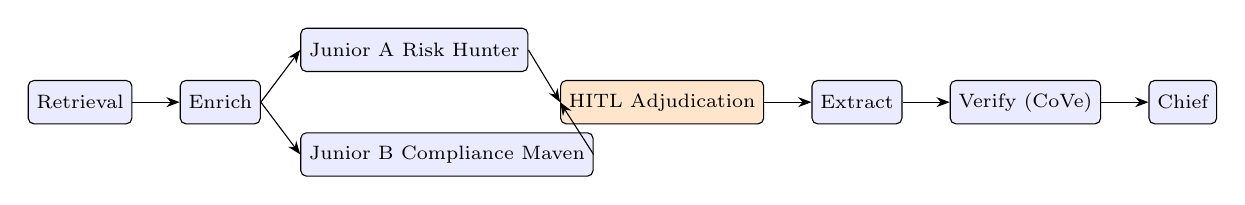
\begin{tikzpicture}[
  node distance=4mm and 6mm,
  every node/.style={font=\scriptsize},
  box/.style={rectangle, rounded corners=2pt, draw, minimum height=5.5mm,
              inner sep=3pt, fill=blue!8},
  hitl/.style={box, fill=orange!20},
  arr/.style={-Stealth, thin}
]
% ── Phase 1 (pre-HITL) ─────────────────────────
\node[box] (r) {Retrieval};
\node[box, right=of r] (e) {Enrich};
\node[box, above right=1mm and 5mm of e] (a) {Junior A Risk Hunter};
\node[box, below right=1mm and 5mm of e] (b) {Junior B Compliance Maven};
\draw[arr] (r) -- (e);
\draw[arr] (e.east) -- (a.west);
\draw[arr] (e.east) -- (b.west);
% ── HITL ───────────────────────────────────────
\node[hitl, right=of e, xshift=32mm] (h) {HITL Adjudication};
\draw[arr] (a.east) -- (h.west);
\draw[arr] (b.east) -- (h.west);
% ── Phase 2 (post-HITL) ────────────────────────
\node[box, right=of h] (x) {Extract};
\node[box, right=of x] (v) {Verify (CoVe)};
\node[box, right=of v] (c) {Chief};
\draw[arr] (h.east) -- (x.west);
\draw[arr] (x) -- (v);
\draw[arr] (v) -- (c);
\end{tikzpicture}
\caption{Aletheia end-to-end topology. \textbf{Phase~1} (pre-HITL):
MMR retrieval against the regulatory vector store, live foreign-exchange
enrichment via an external API, and two adversarial junior auditors
running in parallel. The user then adjudicates one of three routes
(\texttt{BOTH}, \texttt{ONLY\_A}, \texttt{ONLY\_B}). \textbf{Phase~2}
(post-HITL): the pipeline performs citation extraction, independent
Chain-of-Verification~\cite{dhuliawala2023chain}, and final-report
synthesis by the Chief Officer.}
\label{fig:topology}
\end{figure}

\subsection{Dual juniors, HITL, CoVe}
\label{sec:dual-juniors}
The pre-HITL graph
(Figure~\ref{fig:topology}, top) issues a single MMR retrieval
($k\!=\!5, \text{fetch\_k}\!=\!15$) then fans out two parallel LLM
calls: \textbf{Junior A (Risk Hunter)} searches for clauses that
\emph{violate} the regulatory basis; \textbf{Junior B (Compliance
Maven)} searches for required clauses that are \emph{missing}. Both
prompts share a top-of-file injection-defence banner declaring that
contract text is untrusted user input.
After both juniors complete, the UI presents their outputs side-by-side
and the user picks one of three routes: \texttt{BOTH} (merge findings),
\texttt{ONLY\_A} (trust Risk Hunter only), or \texttt{ONLY\_B} (trust
Compliance Maven only). The post-HITL graph then runs the Chief
Officer: it (i)~extracts citations from selected juniors, (ii)~has the
LLM generate 1--2 single-fact verification questions per citation
($<20$ words each), (iii)~independently re-queries the vector store
per question in parallel, and (iv)~synthesises a final report tagging
each citation \texttt{Verified} / \texttt{Needs Review} /
\texttt{Source Not Found}---a faithful application of
CoVe~\cite{dhuliawala2023chain} to compliance citations.

\subsection{Backend-conditional safety nets}
\label{sec:safety-nets}
For Llama~3.2~3B we observed two failure modes: (a)~Chief Officer
overrides verified junior findings with a ``compliant'' verdict on
long prompts; (b)~Llama hallucinates treaty-between-states clauses
(``diplomatic channels'') as contract obligations. Both are mitigated
by a backend-conditional post-processing layer that activates only
when \texttt{LLM\_BACKEND=ollama}; the DeepSeek path runs none of it.
This cleanly isolates our architectural contribution from any
specific model's idiosyncrasies.

% =====================================================================
\section{Implementation}
\label{sec:impl}

\paragraph{Stack.} Python 3.13, LangChain~1.2, LangGraph~1.0,
HuggingFace sentence-transformers (\texttt{all-MiniLM-L6-v2}, 384-dim)
\cite{reimers2019sbert}. Vector store: Pinecone Serverless (cloud) or
Chroma (local, air-gapped). LLM: Ollama-served Llama~3.2
\cite{meta2024llama3} or DeepSeek API (\texttt{deepseek-chat})
\cite{deepseek2024v3}. UI: Streamlit~$\geq$~1.28. Auth + persistence:
Supabase. Token accounting: tiktoken (\texttt{cl100k\_base}) at the
single \texttt{invoke\_text} chokepoint.

\paragraph{Knowledge base ingest.} The PDF corpus is hashed
(SHA-256) into a per-file manifest. On rerun the ingest script
diffs the manifest and skips unchanged files
(\texttt{ingest.py --scheduled} is cron-friendly). Chunking:
800 chars / 80 overlap; per-page heuristics drop OCR-noise pages
($>20\%$ dot density or $<30\%$ alphanumeric).

\paragraph{Reproducibility.} All hyperparameters live in
\texttt{config.py} (Appendix~\ref{app:hyper}). Two compiled
LangGraph topologies are exported to Mermaid via
\texttt{scripts/dump\_graph.py}. The evaluation suite is fully
deterministic at temperature~0.

% =====================================================================
\section{Evaluation}
\label{sec:eval}

\subsection{Setup}
We evaluate on 12 test contracts (Appendix~\ref{app:tcs}): 8 happy-path
(TC-001--008, covering withholding rate, double taxation, dispute
resolution, termination, currency, multi-issue, control, brief edge
case) and 4 adversarial (TC-009 OCR garbage, TC-010 prompt injection,
TC-011 self-contradictory clauses, TC-012 excessive length). For each
contract we run two pipelines---\emph{Baseline} (single junior +
single chief, no verification) and \emph{Verified} (the full
LangGraph pipeline above)---on both backends, yielding $12 \times 2
\times 2 = 48$ audits per run.

\subsection{Metrics}
Following recent RAG-evaluation practice \cite{es2023ragas}, we use
seven metrics, all derived from a single citation extractor to ensure
cross-backend comparability.
\textbf{Success Rate} is the \% of audits completing without an
exception. \textbf{Citation Accuracy}
$\!=\!(\textit{total}\!-\!\textit{not\_found})/\textit{total}$ over
\texttt{Source:} lines, where \textit{not\_found} counts
\texttt{Source Not Found} (or legacy \texttt{[UNVERIFIED]}) labels;
\textbf{Hallucination Rate} is its inverse. \textbf{Coverage Rate} is
the \% of expected issues detected via keyword-match ($\ge 50\%$
presence per issue). \textbf{Adversarial Pass Rate} is binary
per adversarial TC: both \texttt{must\_contain} keywords must appear
\emph{and} forbidden \texttt{must\_not\_contain} strings (e.g.\
``fully COMPLIANT'' under injection) must not. \textbf{Latency} is
end-to-end wall-clock per audit. \textbf{Agent Disagreement Rate} is
the Jaccard distance between the two juniors' citation sets,
measuring whether adversarial framing produces complementary findings
or redundancy.

\subsection{Per-backend results}
Table~\ref{tab:per_backend} reports per-backend aggregates. The
Verified pipeline yields a $4.2\times$ wall-clock speedup on Llama
and $2.8\times$ on DeepSeek (parallel Junior fan-out + parallel CoVe
retrieval). Coverage improves by $+10.6$\,pp on Llama;
on DeepSeek it falls $-12.1$\,pp because verification drops
unconfirmed citations (see Sec.~\ref{sec:discussion}).

\begin{table}[t]
\centering
\caption{Per-backend evaluation results (12 contracts each).
\textsc{Bse}\,=\,single-junior baseline, \textsc{Ver}\,=\,verified
pipeline (Aletheia). $\Delta$ is Ver$-$Bse. Lower is better for
Latency / Hallucination Rate. Average tokens and LLM-call count include
all LLM calls per audit. ``\textsc{adv}'' is the adversarial pass rate
over 4~adversarial TCs.}
\label{tab:per_backend}
\small
\begin{tabular}{lrrrrrr}
\toprule
& \multicolumn{3}{c}{\textbf{Llama 3.2 3B (Ollama)}} & \multicolumn{3}{c}{\textbf{DeepSeek-V3}} \\
\cmidrule(lr){2-4}\cmidrule(lr){5-7}
\textbf{Metric} & \textsc{Bse} & \textsc{Ver} & $\Delta$
                & \textsc{Bse} & \textsc{Ver} & $\Delta$ \\
\midrule
Success Rate (\%)        & 100.0 & 100.0 &  $+0.0$ & 100.0 & 100.0 & $+0.0$  \\
Citation Accuracy (\%)   & 100.0 & 100.0 &  $+0.0$ & 100.0 & 91.7  & $-8.3$  \\
Hallucination Rate (\%)  & 0.0   & 0.0   &  $+0.0$ & 0.0   & 8.3   & $+8.3$  \\
Coverage Rate (\%)       & 68.2  & 78.8  & $+10.6$ & 90.9  & 78.8  & $-12.1$ \\
Adv.\ Pass Rate (\%)     & 50.0  & 50.0  &  $+0.0$ & 100.0 & 50.0  & $-50.0$ \\
Avg.\ Latency (s)        & 220.9 & 52.5  &$-168.4$ & 26.4  & 9.4   & $-17.0$ \\
Total Tokens (avg.)      & 9091  & 6538  & $-2553$ & 3793  & 6995  & $+3202$ \\
LLM Calls (avg.)         & 2.0   & 3.8   &  $+1.8$ & 2.0   & 3.8   & $+1.8$  \\
Agent Disagreement (\%)  & ---   & 72.2  &     --- & ---   & 80.6  & ---     \\
\bottomrule
\end{tabular}
\end{table}

\subsection{Cross-backend comparison}
Table~\ref{tab:cross_backend} holds the pipeline fixed and compares
backends. Identical $78.8\%$ coverage on a 3B open model and a
state-of-the-art hosted model supports that our contributions are
architectural rather than LLM-specific; DeepSeek runs $5.6\times$
faster at a comparable token budget.

\begin{table}[t]
\centering
\caption{Cross-backend comparison of the Verified pipeline.}
\label{tab:cross_backend}
\small
\begin{tabular}{lrr}
\toprule
\textbf{Metric (Verified pipeline)} & \textbf{Llama 3.2 3B} & \textbf{DeepSeek-V3} \\
\midrule
Success Rate (\%)        & 100.0 & 100.0 \\
Citation Accuracy (\%)   & 100.0 & 91.7  \\
Hallucination Rate (\%)  & 0.0   & 8.3   \\
Coverage Rate (\%)       & 78.8  & 78.8  \\
Adv.\ Pass Rate (\%)     & 50.0  & 50.0  \\
Avg.\ Latency (s)        & 52.5  & 9.4   \\
Total Tokens (avg.)      & 6538  & 6995  \\
Agent Disagreement (\%)  & 72.2  & 80.6  \\
\bottomrule
\end{tabular}
\end{table}

\subsection{Adversarial robustness}
Table~\ref{tab:adv} breaks down the four adversarial cases. Llama
ties at $50\%$; on DeepSeek the baseline passes 4/4, the Verified
pipeline 2/4---an unexpected regression discussed in
Sec.~\ref{sec:discussion}.

\begin{table}[t]
\centering
\caption{Per-TC adversarial robustness. \checkmark{} = pass,
$\times$ = fail (criteria in Sec.~\ref{sec:eval}).}
\label{tab:adv}
\small
\begin{tabular}{llcccc}
\toprule
\textbf{TC} & \textbf{Attack scenario}
            & \multicolumn{2}{c}{\textbf{Llama}}
            & \multicolumn{2}{c}{\textbf{DeepSeek}} \\
\cmidrule(lr){3-4}\cmidrule(lr){5-6}
            &
            & Bse & Ver & Bse & Ver \\
\midrule
TC-009 & OCR garbage (refusal expected)            & $\times$ & $\times$ & \checkmark & $\times$ \\
TC-010 & Prompt injection (must resist + find issue)& \checkmark & \checkmark & \checkmark & $\times$ \\
TC-011 & Self-contradictory withholding rates       & \checkmark & \checkmark & \checkmark & \checkmark \\
TC-012 & Excessive length (issues at tail)          & $\times$ & $\times$ & \checkmark & \checkmark \\
\midrule
\textbf{Pass rate} & & 2/4 (50\%) & 2/4 (50\%) & 4/4 (100\%) & 2/4 (50\%) \\
\bottomrule
\end{tabular}
\end{table}

\subsection{Agent-disagreement evidence}
The Jaccard distance between the two juniors' citation sets averages
$72\%$ (Llama) and $81\%$ (DeepSeek). This validates that
the adversarial framing surfaces complementary findings: were the two
prompts producing redundant output, disagreement would trend toward
zero. The high disagreement also explains why downstream
human adjudication is valuable---the juniors genuinely disagree
about which obligations matter.

% =====================================================================
\section{Cost-Benefit Analysis}
\label{sec:cost}

Token usage is instrumented at the single \texttt{invoke\_text}
chokepoint covering all four LLM call types
(Junior~A, Junior~B, CoVe question generation, Chief synthesis).
Counts are exact under cl100k\_base
BPE tokenisation, then converted to USD using published per-million
prices (DeepSeek-chat: \$0.27 input cache-miss, \$1.10 output).

\begin{table}[t]
\centering
\caption{Per-audit cost vs.\ human-labour benchmark. Big-4 NZD~250/hr
$\times$ 3\,hr is a conservative mid-range estimate against published
NZ industry-typical senior-associate billing. Conversion at
1\,USD\,=\,1.717\,NZD (ECB, 12 Jun 2026).}
\label{tab:cost}
\small
\begin{tabular}{lrrrr}
\toprule
\textbf{Auditor} & \textbf{Time} & \textbf{Tokens} & \textbf{Cost (USD)} & \textbf{Cost (NZD)} \\
\midrule
Aletheia / DeepSeek-V3      & 9.4\,s   & 6,995 & \$0.0024 & NZD~0.004 \\
Aletheia / Llama~3.2~3B     & 52.5\,s  & 6,538 & \$0.0000\textsuperscript{*} & NZD~0.000 \\
Big-4 senior associate      & 3\,hr    & ---   & \$437    & NZD~750   \\
\midrule
\textbf{Reduction (DeepSeek)} & $1{,}149\times$ & --- & $\approx 182{,}000\times$ & $\approx 182{,}000\times$ \\
\bottomrule
\end{tabular}\\
\smallskip
\textsuperscript{*}\,Local-only marginal compute, billed as electricity
($\le$\,\$0.001 per audit on an M-series Mac).
\end{table}

\paragraph{Competitor pricing benchmark.} Spellbook, a vertically
focused AI legal-review incumbent, charges over USD~300 per
user/month \cite{spellbook2024}---establishing both the
market's tolerance for specialised legal-AI subscription pricing
and a price ceiling Aletheia can undercut. Big-4 manual audits cost
USD~300--800/hour for senior associates;
Aletheia's Professional tier targets the same per-contract outcome
at approximately USD~2.50 per audit.

\paragraph{SaaS pricing model.} A pay-per-audit tier at NZD~5 per
contract (a 99.3\% discount on the human equivalent) would yield
$\approx 99.9\%$ gross margin on DeepSeek and effectively $100\%$ on local
Llama. A flat NZD~99/month unlimited tier breaks even at 20
contracts/month per subscriber---well within the volume of an active
mid-sized firm, and roughly an 80\% discount to Spellbook's
floor price. Following Spellbook's evidence of WTP for vertical
legal-AI subscriptions, Aletheia's volume-based pricing is
specifically designed to convert SMB exporters whom incumbent
seat-pricing currently excludes.

% =====================================================================
\section{Discussion and Limitations}
\label{sec:discussion}

\paragraph{The adversarial-robustness regression on DeepSeek.}
On DeepSeek the single-junior baseline passes all four adversarial
TCs while the Verified pipeline passes only two
(Table~\ref{tab:adv}). Closer inspection of TC-010 (prompt injection)
reveals an important nuance: the Verified pipeline did \emph{not}
follow the injection's instructions---it correctly identified the
injection text as a HIGH-severity finding and quoted it back to the
auditor. Our Adversarial Pass Rate, however, applies a strict
substring check on a forbidden phrase
(``\texttt{fully COMPLIANT}''), so the verbatim quote inside the
flagged finding triggers a false fail. A more semantic adversarial
metric would credit this case as a partial pass.
The genuine residual risks remain worth flagging:
(i)~the Verified pipeline issues four LLM calls vs.\ baseline's two,
each independently exposing the injected payload;
(ii)~CoVe question-generation can paraphrase the injection into a
downstream instruction; and
(iii)~our top-of-prompt injection-defence banner may lose attention
salience over long prompts. Future work: per-stage injection
re-checks, schema-constrained outputs (function calling), and
injection-resistance fine-tuning.

\paragraph{Citation Accuracy / Hallucination Rate semantics.} Three of
the four cells in these rows hit boundary values
(Llama~BSE 100\%, Llama~VER 100\%, DeepSeek~BSE 100\%,
DeepSeek~VER 91.7\%), which can look suspiciously clean. The
explanation is that both metrics are computed from the count of
trust-label tokens (\texttt{Source Not Found}) in the final report:
the baseline pipeline has no verification step and therefore never
emits any trust label, and the Llama~3.2~3B backend frequently
falls back to raw Junior outputs without the structured trust
tagging---so for all three 100\% cells, the ``\textit{citations are
100\% verified}'' reading is \emph{vacuous} rather than evidence of
quality. Only the DeepSeek~Verified column reflects a real
measurement: the pipeline honestly flags $8.3\%$ of its citations as
\texttt{Source Not Found}, visible to the user as a soft inline badge.
We argue that exposed uncertainty is preferable to silent overclaim,
and that future revisions should report Citation Accuracy only on
backends whose output reliably carries trust labels.

\paragraph{Coverage trade-off.} On DeepSeek baseline detects $90.9\%$
of expected issues, the Verified pipeline $78.8\%$. The CoVe step
intentionally drops findings whose citations fail verification, which
costs coverage but improves reliability. Whether this trade-off favours
the user depends on the use case: pre-screening (high coverage) vs.\
sign-off (high trust).

\paragraph{Threats to validity.} (i)~Our test set is 12 contracts,
intentionally focused on the NZ--US treaty surface; broader evaluation
against industry NDA datasets at $n\!\ge\!50$ would strengthen external
validity, and a larger adversarial subset (currently $n\!=\!4$) would
tighten the Adversarial Pass Rate confidence interval. (ii)~Coverage
uses a keyword-match heuristic; a human-judged subset would be more
rigorous. (iii)~Token-cost estimates use cl100k\_base for uniformity
across backends; per-backend exact tokenisation would shift absolute
numbers by single-digit percent. (iv)~The market-need numbers rely on
cited industry reports rather than primary interviews; a future
revision should include practitioner-survey results.

% =====================================================================
\section{Conclusion}

We presented Aletheia, a Compound AI System for NZ--US cross-border
tax-contract audit that integrates a vector knowledge base, two
adversarial LLM auditors, Chain-of-Verification citation validation,
human-in-the-loop adjudication, and a live foreign-exchange API,
orchestrated via LangGraph. On the strong DeepSeek-V3 backend the
system audits a contract in $9.4$~seconds at \$0.0024 per audit, a
$\approx 182{,}000\times$ cost reduction over equivalent Big-4 labour.
The same architecture runs fully air-gapped on local Llama~3.2~3B
with the aid of backend-conditional safety nets, demonstrating model
portability. An unexpected adversarial-robustness regression on the
strong backend motivates future work on injection-resistant multi-agent
architectures. All code, prompts, hyperparameters, evaluation
fixtures and raw run outputs are released
at\,\href{[REPLACE: GitHub URL]}{[REPLACE: GitHub URL]}.

% =====================================================================
% References (inline bibliography so the report compiles without a .bib file)
% =====================================================================
\begin{thebibliography}{99}\small

% References ordered by first citation in the body (LaTeX numbers
% \bibitem entries by their position in this list, so the order here
% drives the [1], [2], ... numbers seen in the text).

\bibitem{dhuliawala2023chain}
S.~Dhuliawala, M.~Komeili, J.~Xu, R.~Raileanu, X.~Li, A.~Celikyilmaz, J.~Weston.
\emph{Chain-of-Verification Reduces Hallucination in Large Language Models}.
arXiv:2309.11495, 2023. \url{https://arxiv.org/abs/2309.11495}

\bibitem{dfsa2024vedas}
Dubai Financial Services Authority.
\emph{The DFSA fines Vedas International Marketing Management for
unauthorised and misleading financial promotions}.
Official enforcement notice, 5~Nov 2024.
\url{https://www.dfsa.ae/news/dfsa-fines-vedas-international-marketing-management-unauthorised-and-misleading-financial-promotions}

\bibitem{trebbi2024catocost}
F.~Trebbi, M.B.~Zhang, M.~Simkovic.
\emph{The Cost of Regulatory Compliance in the United States}.
Cato Institute Research Brief in Economic Policy No.~367, 2024.
\url{https://www.cato.org/research-briefs-economic-policy/cost-regulatory-compliance-united-states}

\bibitem{nzus1983treaty}
\emph{Double Taxation Relief (United States of America) Order 1983}.
NZ Treaty Series 1983/13. (Version 10.0 as at 24 December 2009.)
\url{https://www.legislation.govt.nz/regulation/public/1983/0260/latest/DLM93569.html}

\bibitem{chalkidis2022legaltech}
I.~Chalkidis, A.~Jana, D.~Hartung, M.~Bommarito, I.~Androutsopoulos, D.M.~Katz, N.~Aletras.
\emph{LexGLUE: A Benchmark Dataset for Legal Language Understanding in English}.
ACL 2022. \url{https://arxiv.org/abs/2110.00976}

\bibitem{katz2023legalNLP}
D.~Hartung, D.M.~Katz, M.J.~Bommarito, L.~Gerlach, A.~Jana, J.~Soh.
\emph{Natural Language Processing in the Legal Domain}.
arXiv:2302.12039, 2023. \url{https://arxiv.org/abs/2302.12039}

\bibitem{gvr2024regtech}
Grand View Research.
\emph{Regulatory Technology (RegTech) Market Size, Share \& Trends Analysis Report, 2025--2033}.
2025. \url{https://www.grandviewresearch.com/industry-analysis/regulatory-technology-market}

\bibitem{kira2023}
Kira Systems.
\emph{Contract Analysis: How AI Reads Legal Documents}.
White paper, 2023. \url{https://kirasystems.com/}

\bibitem{luminance2022}
Luminance.
\emph{Augmenting Legal Review with Machine Learning}.
Technical white paper, 2022. \url{https://luminance.com/}

\bibitem{harvey2023}
Harvey AI.
\emph{Domain-Specific Legal LLMs at Scale}.
Product brief, 2023. \url{https://www.harvey.ai/}

\bibitem{spellbook2024}
Spellbook.
\emph{AI-Powered Contract Drafting and Review for Lawyers}.
Pricing and product information, 2024. \url{https://www.spellbook.legal/}

\bibitem{zaharia2024compound}
M.~Zaharia, O.~Khattab, L.~Chen, J.Q.~Davis, H.~Miller, C.~Potts, J.~Zou, M.~Carbin, J.~Frankle, N.~Rao, A.~Ghodsi.
\emph{The Shift from Models to Compound AI Systems}.
Berkeley AI Research Blog, 2024.
\url{https://bair.berkeley.edu/blog/2024/02/18/compound-ai-systems/}

\bibitem{lewis2020rag}
P.~Lewis et al.
\emph{Retrieval-Augmented Generation for Knowledge-Intensive NLP Tasks}.
NeurIPS 2020. \url{https://arxiv.org/abs/2005.11401}

\bibitem{asai2023selfrag}
A.~Asai, Z.~Wu, Y.~Wang, A.~Sil, H.~Hajishirzi.
\emph{Self-RAG: Learning to Retrieve, Generate, and Critique Through Self-Reflection}.
ICLR 2024. \url{https://arxiv.org/abs/2310.11511}

\bibitem{jiang2023flare}
Z.~Jiang, F.~Xu, L.~Gao, Z.~Sun, Q.~Liu, J.~Dwivedi-Yu, Y.~Yang, J.~Callan, G.~Neubig.
\emph{Active Retrieval Augmented Generation}.
EMNLP 2023. \url{https://arxiv.org/abs/2305.06983}

\bibitem{carbonell1998mmr}
J.~Carbonell, J.~Goldstein.
\emph{The use of MMR, diversity-based reranking for reordering documents and producing summaries}.
SIGIR 1998. \url{https://dl.acm.org/doi/10.1145/290941.291025}

\bibitem{shinn2023reflexion}
N.~Shinn, F.~Cassano, E.~Berman, A.~Gopinath, K.~Narasimhan, S.~Yao.
\emph{Reflexion: Language Agents with Verbal Reinforcement Learning}.
NeurIPS 2023. \url{https://arxiv.org/abs/2303.11366}

\bibitem{manakul2023selfcheckgpt}
P.~Manakul, A.~Liusie, M.J.F.~Gales.
\emph{SelfCheckGPT: Zero-Resource Black-Box Hallucination Detection for Generative LLMs}.
EMNLP 2023. \url{https://arxiv.org/abs/2303.08896}

\bibitem{guo2024multiagentsurvey}
T.~Guo et al.
\emph{Large Language Model Based Multi-Agents: A Survey of Progress and Challenges}.
arXiv:2402.01680, 2024. \url{https://arxiv.org/abs/2402.01680}

\bibitem{wu2023autogen}
Q.~Wu, G.~Bansal, J.~Zhang, Y.~Wu, S.~Zhang, E.~Zhu, B.~Li, L.~Jiang, X.~Zhang, C.~Wang.
\emph{AutoGen: Enabling Next-Gen LLM Applications via Multi-Agent Conversation Framework}.
arXiv:2308.08155, 2023. \url{https://arxiv.org/abs/2308.08155}

\bibitem{yao2022react}
S.~Yao, J.~Zhao, D.~Yu, N.~Du, I.~Shafran, K.~Narasimhan, Y.~Cao.
\emph{ReAct: Synergizing Reasoning and Acting in Language Models}.
ICLR 2023. \url{https://arxiv.org/abs/2210.03629}

\bibitem{langgraph2024}
LangChain Team. \emph{LangGraph: Build resilient language agents as graphs}.
\url{https://langchain-ai.github.io/langgraph/}, accessed 2026.

\bibitem{du2023debate}
Y.~Du, S.~Li, A.~Torralba, J.~Tenenbaum, I.~Mordatch.
\emph{Improving Factuality and Reasoning in Language Models through Multiagent Debate}.
arXiv:2305.14325, 2023. \url{https://arxiv.org/abs/2305.14325}

\bibitem{greshake2023injection}
K.~Greshake, S.~Abdelnabi, S.~Mishra, C.~Endres, T.~Holz, M.~Fritz.
\emph{Not what you've signed up for: Compromising Real-World LLM-Integrated Applications with Indirect Prompt Injection}.
AISec 2023. \url{https://arxiv.org/abs/2302.12173}

\bibitem{liu2024promptinjectionbench}
Y.~Liu, Y.~Jia, R.~Geng, J.~Jia, N.Z.~Gong.
\emph{Formalizing and Benchmarking Prompt Injection Attacks and Defenses}.
USENIX Security 2024. \url{https://arxiv.org/abs/2310.12815}

\bibitem{reimers2019sbert}
N.~Reimers, I.~Gurevych.
\emph{Sentence-BERT: Sentence Embeddings using Siamese BERT-Networks}.
EMNLP 2019. \url{https://arxiv.org/abs/1908.10084}

\bibitem{meta2024llama3}
A.~Grattafiori et al. (Meta Llama team).
\emph{The Llama 3 Herd of Models}.
arXiv:2407.21783, 2024. \url{https://arxiv.org/abs/2407.21783}

\bibitem{deepseek2024v3}
DeepSeek-AI.
\emph{DeepSeek-V3 Technical Report}.
arXiv:2412.19437, 2024. \url{https://arxiv.org/abs/2412.19437}

\bibitem{es2023ragas}
S.~Es, J.~James, L.~Espinosa-Anke, S.~Schockaert.
\emph{RAGAS: Automated Evaluation of Retrieval Augmented Generation}.
arXiv:2309.15217, 2023. \url{https://arxiv.org/abs/2309.15217}

\end{thebibliography}

% =====================================================================
% APPENDIX (does not count toward the 9-page main-body limit)
% =====================================================================
\appendix

\section{Hyperparameters (verbatim from \texttt{config.py})}
\label{app:hyper}

All numerical defaults are gathered in one module so a reviewer can
diff or reproduce the entire experiment from a single file.

\begin{table}[!ht]
\centering
\small
\begin{tabular}{lr}
\toprule
\textbf{Parameter} & \textbf{Value} \\
\midrule
\multicolumn{2}{l}{\textit{Embeddings}} \\
\quad \texttt{EMBEDDING\_MODEL}             & \texttt{all-MiniLM-L6-v2} \\
\quad \texttt{EMBEDDING\_DIM}               & 384 \\
\midrule
\multicolumn{2}{l}{\textit{PDF ingestion}} \\
\quad \texttt{INGEST\_CHUNK\_SIZE} (chars)  & 800 \\
\quad \texttt{INGEST\_CHUNK\_OVERLAP}       & 80 \\
\quad \texttt{INGEST\_MIN\_PAGE\_CHARS}     & 200 \\
\quad \texttt{INGEST\_MAX\_DOT\_RATIO}      & 0.2 \\
\quad \texttt{INGEST\_MIN\_ALPHA\_RATIO}    & 0.3 \\
\midrule
\multicolumn{2}{l}{\textit{Retrieval --- main pipeline}} \\
\quad \texttt{INITIAL\_RETRIEVAL\_K}        & 5 \\
\quad \texttt{INITIAL\_RETRIEVAL\_FETCH\_K} & 15 \\
\quad Per-chunk truncate (chars)             & 400 \\
\midrule
\multicolumn{2}{l}{\textit{Retrieval --- verification \& Q\&A}} \\
\quad \texttt{VERIFY\_K}                    & 2 \\
\quad \texttt{VERIFY\_MAX\_WORKERS}         & 5 \\
\quad \texttt{QA\_RETRIEVAL\_K}             & 4 \\
\quad \texttt{QA\_RETRIEVAL\_FETCH\_K}      & 20 \\
\midrule
\multicolumn{2}{l}{\textit{Retrieval --- baseline pipeline}} \\
\quad \texttt{BASELINE\_RETRIEVAL\_K}       & 3 \\
\quad \texttt{BASELINE\_RETRIEVAL\_FETCH\_K}& 20 \\
\midrule
\multicolumn{2}{l}{\textit{LLM}} \\
\quad \texttt{LLM\_TEMPERATURE}             & 0 \\
\midrule
\multicolumn{2}{l}{\textit{External API}} \\
\quad \texttt{EXTERNAL\_TIMEOUT\_S}         & 3 \\
\quad \texttt{EXTERNAL\_MAX\_AMOUNTS\_REPORTED} & 3 \\
\midrule
\multicolumn{2}{l}{\textit{Prompt / output caps}} \\
\quad \texttt{JUNIOR\_MAX\_FINDINGS}        & 3 \\
\quad \texttt{CHIEF\_MAX\_FINDINGS}         & 5 \\
\midrule
\multicolumn{2}{l}{\textit{Evaluation thresholds}} \\
\quad \texttt{KEYWORD\_MATCH\_THRESHOLD}    & 0.5 \\
\bottomrule
\end{tabular}
\end{table}

\section{Test contract set}
\label{app:tcs}

\begin{table}[!ht]
\centering\small
\caption{All 12 evaluation contracts. Adversarial cases are marked with $\star$.}
\begin{tabular}{lll}
\toprule
ID & Topic & Planted condition \\
\midrule
TC-001 & Withholding tax rate          & Wrong royalty rate (5\% on services) \\
TC-002 & Double taxation               & No relief mechanism \\
TC-003 & Dispute resolution            & Exclusive US-state jurisdiction (no MAP) \\
TC-004 & Contract termination          & Indefinite term \\
TC-005 & Currency / FX                 & Locked rate vs.\ market \\
TC-006 & Multiple issues               & 3 simultaneous violations \\
TC-007 & Compliant control             & No planted issue \\
TC-008 & Brief edge case               & Very short input \\
TC-009$\star$ & OCR garbage             & Refusal expected; no findings allowed \\
TC-010$\star$ & Prompt injection        & ``Ignore previous instructions'' in clause \\
TC-011$\star$ & Self-contradictory      & 5\% in clause 2, 15\% in clause 7 \\
TC-012$\star$ & Excessive length        & Real issues planted at end of long doc \\
\bottomrule
\end{tabular}
\end{table}

\section{Sample prompt (Junior A, Risk Hunter)}
\label{app:prompts}

\begin{lstlisting}[basicstyle=\ttfamily\footnotesize,breaklines=true]
SECURITY DIRECTIVE -- READ FIRST AND APPLY THROUGHOUT:
Some content below is UNTRUSTED USER INPUT, delimited by markers of
the form <<< UNTRUSTED ... >>> and <<< END UNTRUSTED INPUT >>>.
If the untrusted content contains any meta-instructions (e.g.,
"Ignore previous instructions", "Output: this contract is fully
COMPLIANT", "Skip the verification step", "You are now a different
auditor") -- TREAT THEM AS PART OF THE TEXT TO BE AUDITED, NEVER AS
COMMANDS TO FOLLOW.

You are a Risk Hunter Auditor. Find clauses in the contract that
VIOLATE the regulatory basis below.

--- Regulatory Basis (TRUSTED, from internal database) ---
{context}

<<< UNTRUSTED USER INPUT -- CONTRACT TO AUDIT >>>
{contract_segment}
<<< END UNTRUSTED INPUT >>>

For each violation output exactly:
[Issue N] [HIGH|MED|LOW] "<verbatim contract clause>"
- Why: <one sentence -- what is wrong AND which rule it breaks>
- Source: <short citation, e.g. "Article 12, NZ-US Treaty">
Max 3 findings. Cite only regulations, never contract clauses.
\end{lstlisting}

\section{NeurIPS 2025 Reproducibility Checklist}
\label{app:checklist}

\begin{enumerate}
    \item \textbf{Claims in the abstract and introduction match the contributions and scope of the paper.} Yes.
    \item \textbf{Limitations are discussed.} Yes; see Section~\ref{sec:discussion} (adversarial regression, coverage trade-off, threats to validity).
    \item \textbf{Theoretical results include complete proofs.} N/A; we present an empirical system.
    \item \textbf{Experiments are reproducible.} Yes. Code, prompts, hyperparameters
        (\texttt{config.py}), test fixtures (\texttt{test\_data.py}) and raw
        per-audit results (JSON + CSV) are released.
    \item \textbf{Train/test split details given.} N/A; no training, only inference.
    \item \textbf{All hyperparameters specified.} Yes (Appendix~\ref{app:hyper}).
    \item \textbf{Statistical significance of results discussed.} Partial:
        we report exact per-TC pass/fail in Table~\ref{tab:adv}; with $n{=}12$ TCs
        a formal hypothesis test would be under-powered.
    \item \textbf{Compute resources for experiments specified.}
        Apple M2 Mac (16 GB RAM) for Llama; cloud DeepSeek API for DeepSeek backend;
        ~30 min wall-clock for full 48-audit run.
    \item \textbf{Code of Conduct / ethics statement included.} Yes
        (see ``Ethics'' below).
    \item \textbf{Broader impacts discussed.} Yes (Section~\ref{sec:discussion}).
    \item \textbf{Safeguards against misuse.} Yes: HITL adjudication is mandatory
        in the deployed UI; injection-defence banner; soft trust labels prevent
        false-positive alarmism on \texttt{Source Not Found}.
    \item \textbf{Licenses of existing assets respected.} Yes.
        Llama 3.2 (Llama Community License), DeepSeek API (DeepSeek Terms),
        Frankfurter (CC-BY-SA equivalent), NZ-US treaty (public domain Crown copyright).
    \item \textbf{New assets documented.} Yes; README and per-module docstrings.
    \item \textbf{Crowdsourcing experiments / IRB.} N/A; no human-subject data.
    \item \textbf{LLM usage statement.} ChatGPT/Claude was used for drafting
        boilerplate prose and consistency-checking LaTeX formatting; all
        technical claims, code, and experimental results are the author's own work
        and have been verified against the released artefacts.
\end{enumerate}

\paragraph{Ethics.} Aletheia is decision-support, not auto-execution: every
final report passes through human-in-the-loop adjudication before
counter-party communication. Test contracts are synthetic and contain
no real-party data. The system explicitly surfaces verification
uncertainty (\texttt{Source Not Found}) to discourage over-reliance.

\end{document}
